\documentclass[border=4pt]{standalone}
\usepackage{amsmath,amssymb,tikz}\usetikzlibrary{arrows.meta}
\definecolor{figB}{RGB}{31,90,166}\definecolor{figR}{RGB}{176,48,48}\definecolor{figG}{RGB}{46,125,50}\definecolor{figO}{RGB}{214,120,20}
% v1 = (2.2,0), v2 = (0.9,1.3): R_{11} = |v1| = 2.2, R_{22} = dist(v2, span v1) = 1.3 <= |v2| = 1.581
\begin{document}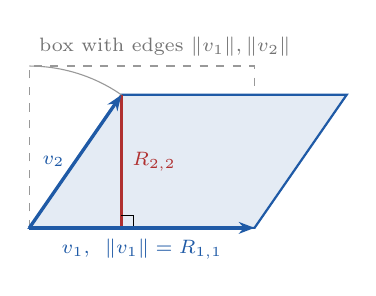
\begin{tikzpicture}[scale=1.3,>={Stealth[length=2mm]}]
\draw[black!40,thin,dashed] (0,0) rectangle (2.2,1.581);
\node[font=\scriptsize,black!55,anchor=south west] at (0,1.581) {box with edges $\|v_1\|,\|v_2\|$};
\fill[figB!12] (0,0)--(2.2,0)--(3.1,1.3)--(0.9,1.3)--cycle;
\draw[thick,figB] (0,0)--(2.2,0)--(3.1,1.3)--(0.9,1.3)--cycle;
\draw[black!40,thin] (0,1.581) arc (90:55.3:1.581);
\draw[very thick,figR] (0.9,0)--(0.9,1.3) node[midway,right,font=\scriptsize]{$R_{2,2}$};
\draw[thin] (0.9,0.12)--(1.02,0.12)--(1.02,0);
\draw[->,very thick,figB] (0,0)--(2.2,0) node[midway,below,font=\scriptsize]{$v_1$, \ $\|v_1\|=R_{1,1}$};
\draw[->,very thick,figB] (0,0)--(0.9,1.3) node[midway,left,font=\scriptsize]{$v_2$};
\end{tikzpicture}\end{document}
